\sloppy
\documentclass[14pt,a4paper,oneside]{extarticle}	% Размер основного шрифта и формата листа
\usepackage{xltxtra}						% Используется для вывода логотипа XeLaTeX
\usepackage{xunicode}						% Кодировка документа
\usepackage{polyglossia}					% Загружает пакет многоязыковой верстки
\newfontfamily\russianfont{Book Antiqua}
%\setmainfont{Liberation Serif}						% Основной шрифт текста
\setmainfont{Book Antiqua}
\setdefaultlanguage{russian}				% Основной язык текста
\setotherlanguage{english}					% Дополнительный язык текста
\linespread{1}							% Межстрочный интервал выбран полуторным
\usepackage[left=2.5cm,
right=1.5cm,vmargin=2.5cm]{geometry} % Отступы по краям листа
\bibliographystyle{ugost2008}

\usepackage{xcolor}
\usepackage{hyperref}
% Цвета для гиперссылок
\definecolor{linkcolor}{HTML}{359B08} % цвет ссылок
\definecolor{urlcolor}{HTML}{799B03} % цвет гиперссылок
\hypersetup{pdfstartview=FitH,  linkcolor=linkcolor,urlcolor=urlcolor, colorlinks=true}

%---------------------------%
%---- Пакеты расширений ----%
%---------------------------%
\usepackage{xcolor}
\usepackage{hyperref}
% Цвета для гиперссылок
\definecolor{linkcolor}{HTML}{359B08} % цвет ссылок
\definecolor{urlcolor}{HTML}{799B03} % цвет гиперссылок
\hypersetup{pdfstartview=FitH,  linkcolor=linkcolor,urlcolor=urlcolor, colorlinks=true}


\usepackage{verbatim,indentfirst}
\usepackage{cite,enumerate,float}
\usepackage{amsmath,amssymb,amsthm,amsfonts}

%---------------------------%
%--- Вставка иллюстраций ---%
%---------------------------%
\usepackage{graphicx}
\usepackage{subfigure}
%\graphicspath{{Images/}}
\usepackage{fontspec}

\begin{document}
%	\pagestyle{empty} %  выключаенм нумерацию
	
	%\setcounter{page}{3}% Нумерация начинается с третьей страницы
	%\renewcommand{\contentsname}{\center{Содержание}}
	%\tableofcontents
	
	\begin{center}
		%\addcontentsline{toc}{section}{Опыт 16. Нахождение центра масс}
		\subsection*{Гироскоп на вращающейся платформе}
	\end{center}
	
	\begin{figure}[H] 	
		\centering 	
		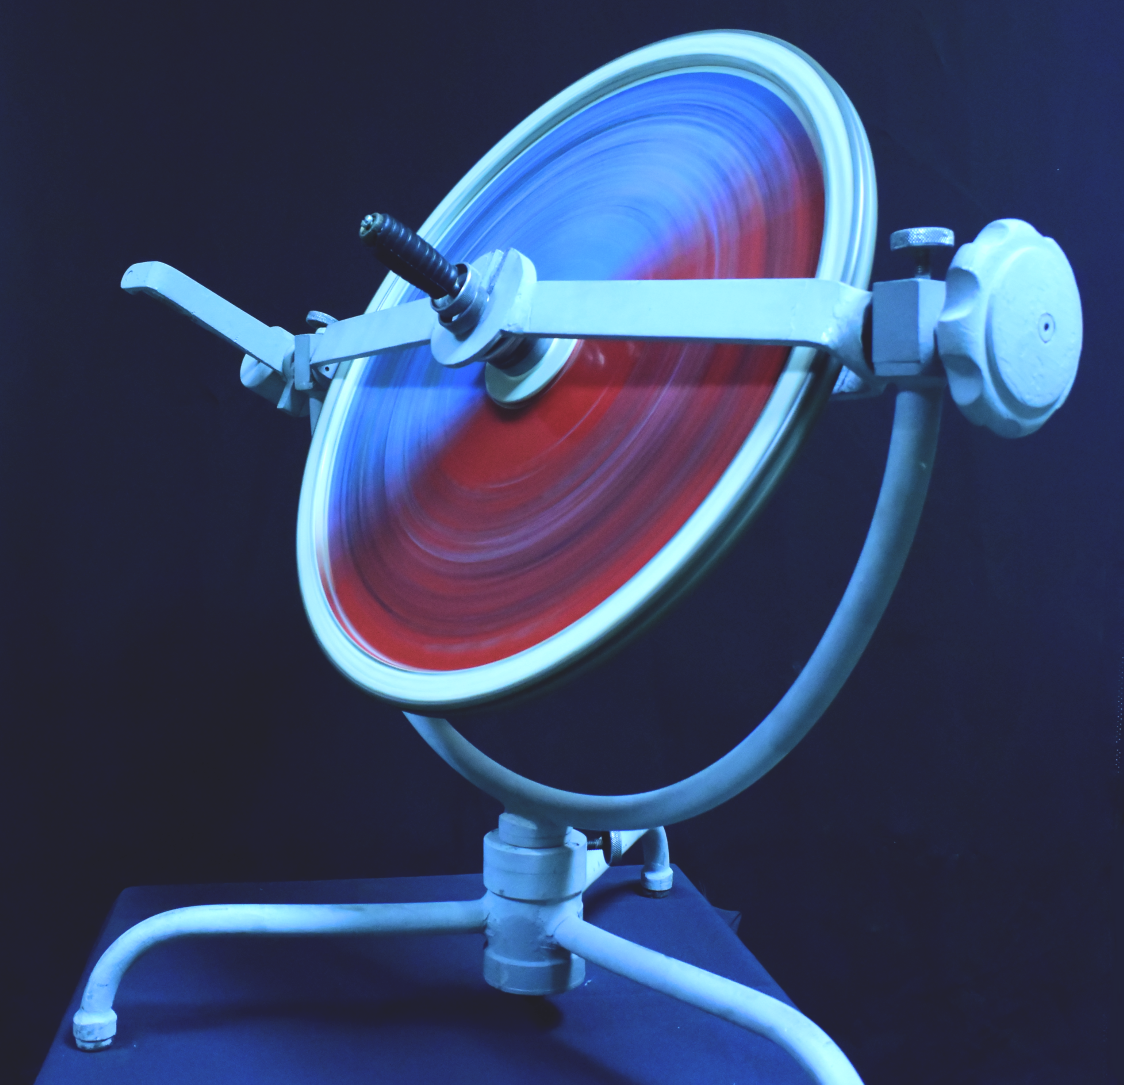
\includegraphics[width=0.75\linewidth]{gyro-1.png}
		\caption{Демонстрация гироскопического эффекта, связанного с сохранением свободным гироскопом неизменного направления оси вращения в пространстве}
		\label{gyro-1}
	\end{figure}
	
	\subsection*{\underline{Оборудование:}}

			\begin{enumerate} 
			\item Гироскоп в кардановом подвесе.
			\item Устройство для раскручивания гироскопа или шнур.
			\item Вращающаяся платформа.
		\end{enumerate}


		\subsection*{\underline{Основные определения:}}
		
		Гироскоп представляет собой массивное твердое тело (в данном случае - диск), способное свободно вращаться вокруг заданной оси. 
		Для обеспечения свободы вращения гироскопа вокруг «неподвижной» точки применяют специальную систему крепления -- карданов подвес (рис.\ref{gyro-1}) .
		В демонстрации с волчком отмечалось, что если центр тяжести гироскопа совпадает с его «неподвижной» точкой (точкой пересечения осей карданова подвеса), то такой гироскоп называется астатическим.
		Астатические гироскопы применяются в качестве измерительных элементов, определяющих заданное направление в пространстве, и, в частности, как временные «хранители» направления истинной вертикали, направления меридиана или ортодромии и являются датчиками автопилота, прицела, антенны, определяющими положение объекта относительно заданного направления в пространстве.
		
		Принцип действия вращающегося астатического гироскопа основан на использовании способности вектора момента импульса \textbf{L} сохранять заданное направление в пространстве при отсутствии внешних моментов.
		Тогда направление оси ротора гироскопа в пространстве служит исходной базой для определения положения движущегося объекта, антенны и проч.
		
		В процессе эксплуатации ось ротора астатического гироскопа, подверженная действию моментов внешних сил, совершает вынужденные колебания и постепенно отклоняется от заданного направления в пространстве.		
		Скорость отклонения оси ротора гироскопа в пространстве называется собственной скоростью прецессии гироскопа $ \Omega $, или просто «уходом», и является наиболее важной характеристикой точности прибора.

	\subsection*{\underline{Краткое описание:}}
	
	Перед началом опыта необходимо убедиться, что винты на приборе затянуты и гироскоп свободно вращается только вокруг своей собственной оси (эта ось проходит через втулку колеса).
	Гироскоп приводят во вращение шнуром, намотанным на ось, или при помощи специального устройства.
	После начала вращения винты ослабляются, и гироскоп становится «свободным», т.е. может вращаться в трех различных плоскостях.
	Затем быстро поворачивают подставку гироскопа вокруг вертикальной оси в ту или другую сторону и показывают, что при этом ось вращающегося гироскопа сохраняет неизменным свое направление в пространстве (рис.\ref{gyro-2}).
	
		\begin{figure}[H]
		\centering 		
		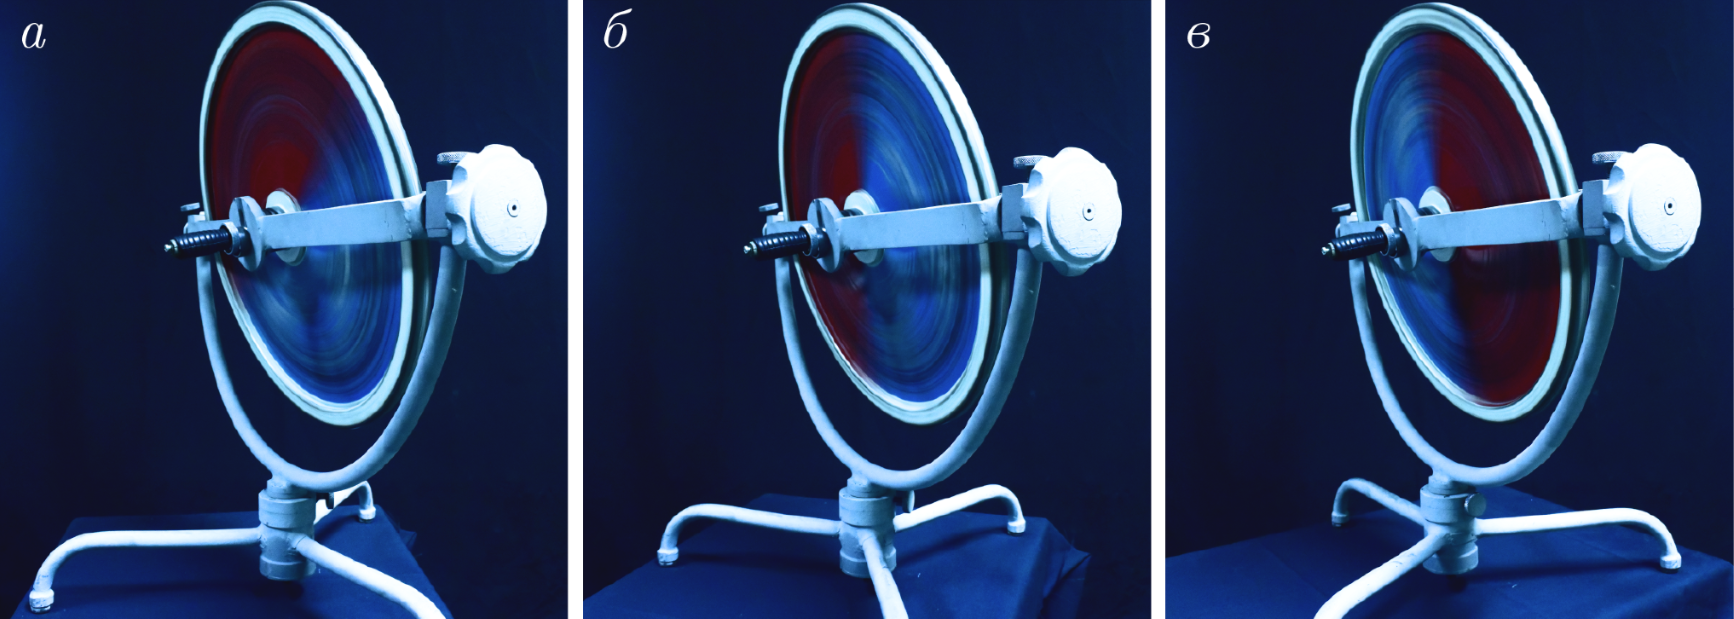
\includegraphics[width=0.9\linewidth]{gyro-2.png}		
		\caption{Демонстрация гироскопического эффекта, связанного с сохранением свободным гироскопом неизменного направления оси вращения в пространстве}
		\label{gyro-2}	
	\end{figure}

Вектор момента импульса, направленный вдоль оси ротора способен сохранять свое положение в пространстве даже при наклоне подставки гироскопа на некоторый угол.
Чем выше скорость вращения или больше момент инерции диска, тем более явно проявляется эта особенность гироскопа.

	\subsection*{\underline{Теория:}}
	
	Для свободного вращающегося гироскопа сила тяжести не может изменить ориентацию его оси вращения, так как эта сила приложена к центру масс (центр вращения в этом случае совпадает с центром масс), а момент силы тяжести относительно закрепленного центра масс равен нулю.
	Поэтому если на гироскоп не действуют никакие другие внешние силы, то, следовательно, отсутствует момент этих сил относительно его закрепленного центра масс.
	Согласно основному закону динамики вращательного движения
\begin{equation}\label{gyro-eq1}
	\frac{\Delta \textbf{L}}{\Delta t} = \textbf{M},
	\end{equation} 
	если $ \textbf{M}=0 $, то $ \textbf{L} = \text{const} $, т. е. момент импульса гироскопа сохраняет свою величину и направление в пространстве.
	Следовательно, вместе с ним сохраняет свое положение в пространстве и ось гироскопа.
		
	Чтобы ось гироскопа изменила свое направление в пространстве, необходимо, согласно основному закону динамики вращательного движения твердого тела (\ref{gyro-eq1}), создать отличный от нуля момент внешних сил.
	Поэтому если момент внешних сил, приложенных к вращающемуся гироскопу относительно его центра масс, не равен нулю, то наблюдается явление, получившее название гироскопического эффекта.
	
	Гироскопический эффект объясняется следующим образом.
	Момент  \textbf{М}, создаваемый парой внешних сил \textbf{F}, направлен вдоль прямой $ O_2 $ (рис.\ref{gyro-3}). 
	За время $ \Delta t $ момент импульса гироскопа получит приращение $$ \Delta \textbf{L} = \textbf{M} \Delta t $$ (направление $ \Delta \textbf{L} $ совпадает с направлением \textbf{M}) и станет равным $$ \textbf{L}_2=\textbf{L}_1+\Delta \textbf{L}. $$
	
	Направление вектора $ \textbf{L}_2 $ совпадает с новым направлением оси вращения гироскопа.
	Таким образом, ось вращения гироскопа повернется вокруг оси $ O_3 $.
	
			\begin{figure}[H]
	\centering 	
	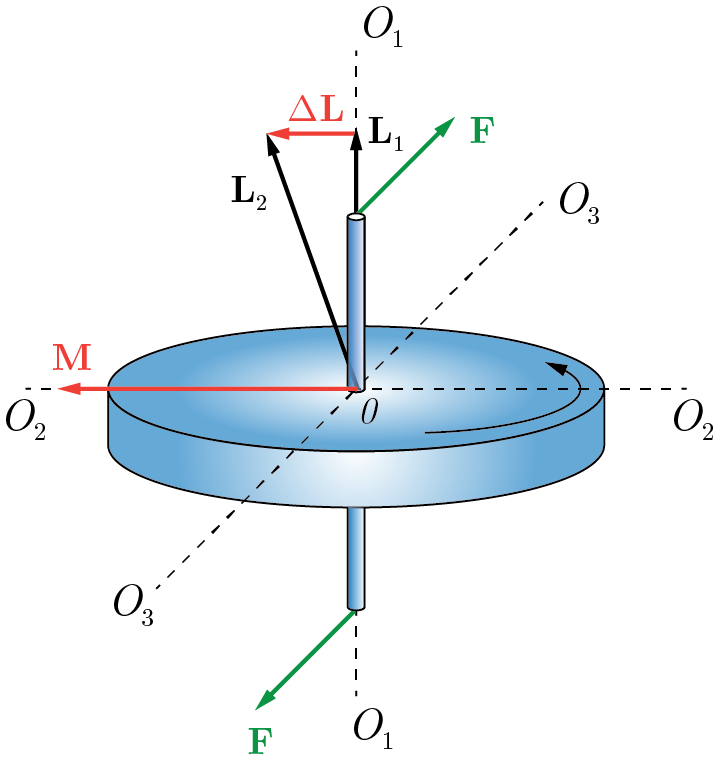
\includegraphics[width=0.6\linewidth]{gyro-3.png}
	\caption{Схематичное изображение динамики вращающегося диска гироскопа. Пара внешних сил \textbf{F}, приложенных к оси вращения тела создает отличный от нуля момент внешних сил \textbf{M}, который поворачивает вектор момента импульса диска $ \textbf{L} $ вокруг оси $ O_3 $}
	\label{gyro-3}
\end{figure}
	
	Если время действия силы мало, то, даже при большом значении момента сил \textbf{М}, изменение момента импульса $ \Delta\textbf{L} $ гироскопа будет очень малым.
	Отсюда следует вывод, что кратковременное действие внешних сил практически не приводит к изменению ориентации оси вращения гироскопа в пространстве.
	Для ее изменения следует прикладывать силы в течение длительного времени.
	
\end{document}
